\subsection{T1 phase of $\ce{Mn3Pt}$}


\begin{figure}[H]
    \centering
    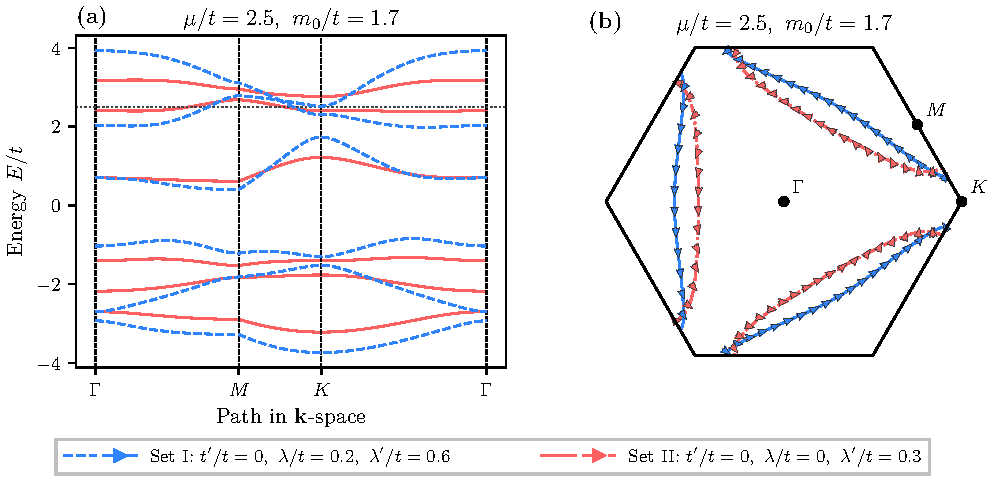
\includegraphics[
        width=\linewidth
    ]{Plots/Mn3Pt T1/Mn3Pt1_special_case.ipynb.pdf}
    \par\bigskip
    \begin{subfigure}[t]{0.48\textwidth}
        \centering
        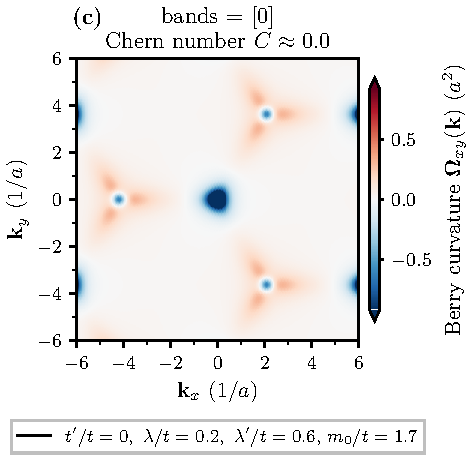
\includegraphics[
            width=\linewidth
        ]{Plots/Mn3Pt T1/Mn3Pt1_special_case.ipynb_berry_wo_soc.pdf}
        
    \end{subfigure}
    \hfill
    \begin{subfigure}[t]{0.48\textwidth}
        \centering
        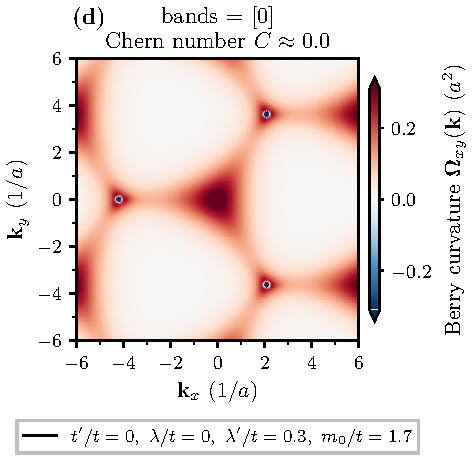
\includegraphics[
            width=\linewidth
        ]{Plots/Mn3Pt T1/Mn3Pt1_special_case.ipynb_berry_w_soc.pdf}
        
    \end{subfigure}
    \caption{Depicted is the (a) Band structure along the high-symmetry points $\Gamma$-$K$-$M$, (b) the in-plane Fermi surface spin textures for the Fermi-level µ and in (c),(d) the computed Berry curvatures for no SOC, or with SOC respectively, for the T1 phase of \ce{Mn3Pt} in the nonbreathing limit.}
    \label{fig:Mn3Pt1-special-case}
\end{figure}


\subsection{T2 phase of $\ce{Mn3Pt}$}




\begin{figure}[H]
    \centering
    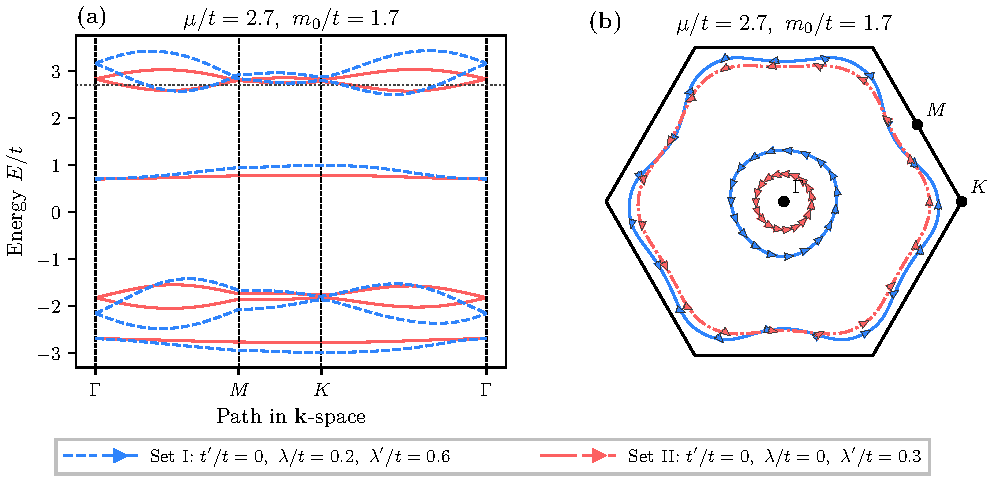
\includegraphics[
        width=\linewidth
    ]{Plots/Mn3Pt T2/Mn3Pt2_special_case.ipynb.pdf}
    \par\bigskip
    \begin{subfigure}[t]{0.48\textwidth}
        \centering
        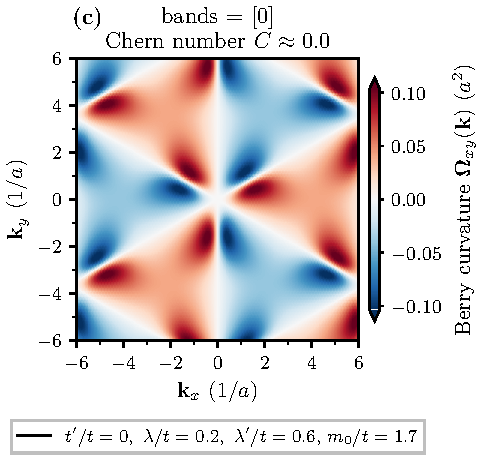
\includegraphics[
            width=\linewidth
        ]{Plots/Mn3Pt T2/Mn3Pt2_special_case.ipynb_berry_wo_soc.pdf}
        
    \end{subfigure}
    \hfill
    \begin{subfigure}[t]{0.48\textwidth}
        \centering
        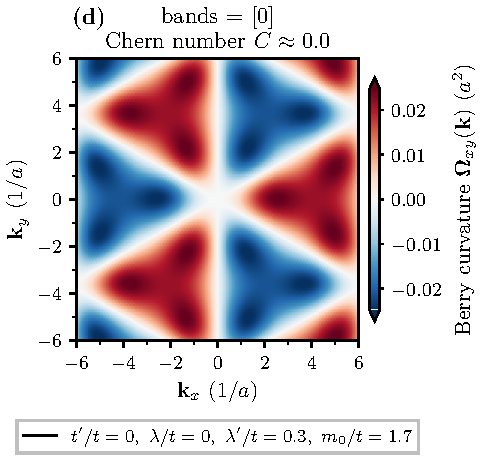
\includegraphics[
            width=\linewidth
        ]{Plots/Mn3Pt T2/Mn3Pt2_special_case.ipynb_berry_w_soc.pdf}
        
    \end{subfigure}
    \caption{Depicted is the (a) Band structure along the high-symmetry points $\Gamma$-$K$-$M$, (b) the in-plane Fermi surface spin textures for the Fermi-level µ and in (c),(d) the computed Berry curvatures for no SOC, or with SOC respectively, for the Pt2 phase of \ce{Mn3Pt} in the nonbreathing limit.}
    \label{fig:Mn3Pt2-special-case}
\end{figure}



\subsection{$\ce{Mn3Ge}$}

\begin{figure}[H]
    \centering
    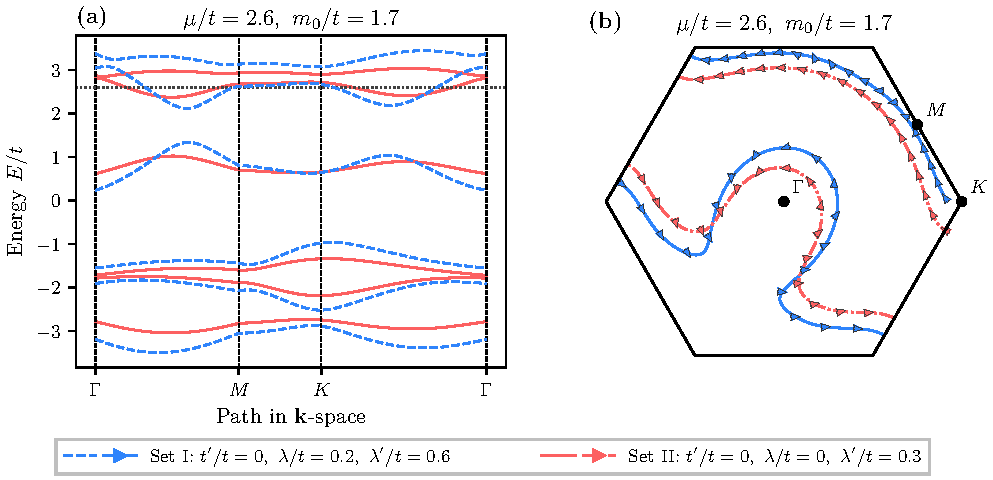
\includegraphics[
        width=\linewidth
    ]{Plots/Mn3Ge/special_case.pdf}
    \par\bigskip
    \begin{subfigure}[t]{0.48\textwidth}
        \centering
        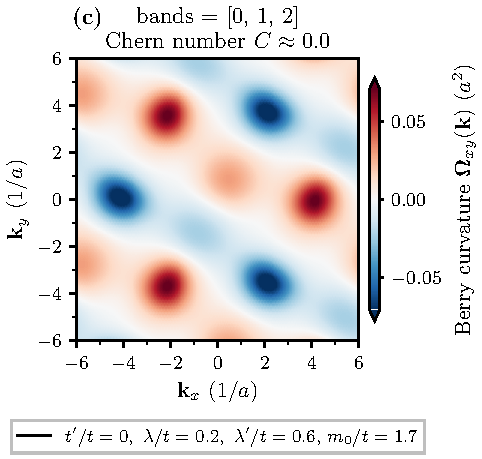
\includegraphics[
            width=\linewidth
        ]{Plots/Mn3Ge/special_case_berry_wo_soc.pdf}
        
    \end{subfigure}
    \hfill
    \begin{subfigure}[t]{0.48\textwidth}
        \centering
        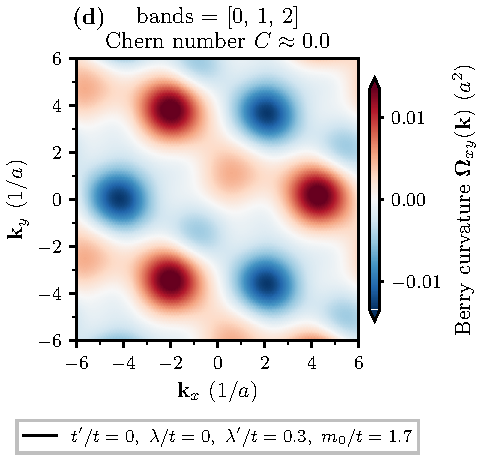
\includegraphics[
            width=\linewidth
        ]{Plots/Mn3Ge/special_case_berry_w_soc.pdf}
        
    \end{subfigure}
    \caption{Depicted is the (a) Band structure along the high-symmetry points $\Gamma$-$K$-$M$, (b) the in-plane Fermi surface spin textures for the Fermi-level µ and in (c),(d) the computed Berry curvatures for no SOC, or with SOC respectively, for the T1 phase of \ce{Mn3Pt} in the nonbreathing limit.}
    \label{fig:Mn3Ge-special-case}
\end{figure}



\subsection{$\ce{Mn3Sn}$}


\begin{figure}[H]
    \centering
    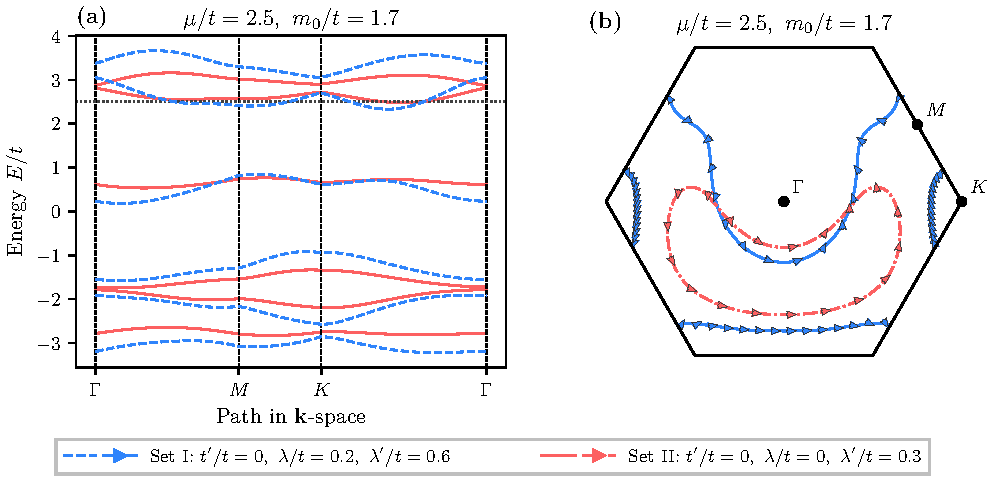
\includegraphics[
        width=\linewidth
    ]{Plots/Mn3Sn/Mn3Sn_special_case.pdf}
    \par\bigskip
    \begin{subfigure}[t]{0.48\textwidth}
        \centering
        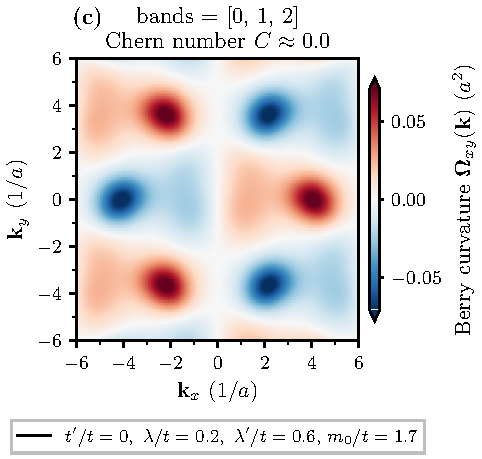
\includegraphics[
            width=\linewidth
        ]{Plots/Mn3Sn/Mn3Sn_special_case_berry_wo_soc.pdf}
        
    \end{subfigure}
    \hfill
    \begin{subfigure}[t]{0.48\textwidth}
        \centering
        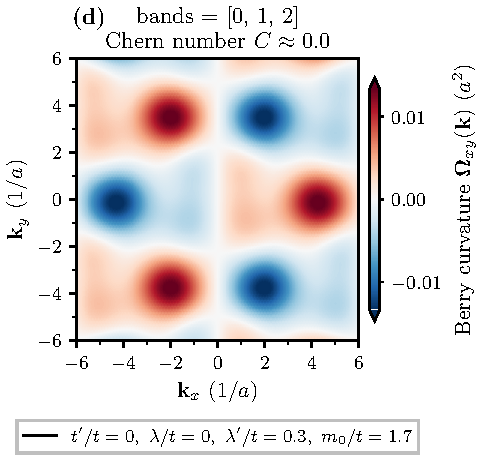
\includegraphics[
            width=\linewidth
        ]{Plots/Mn3Sn/Mn3Sn_special_case_berry_w_soc.pdf}
        
    \end{subfigure}
    \caption{Depicted is the (a) Band structure along the high-symmetry points $\Gamma$-$K$-$M$, (b) the in-plane Fermi surface spin textures for the Fermi-level µ and in (c),(d) the computed Berry curvatures for no SOC, or with SOC respectively, for the T1 phase of \ce{Mn3Pt} in the nonbreathing limit.}
    \label{fig:Mn3Sn-special-case}
\end{figure}
